\section{Staggering the three extraction stages}\label{sec:stagger}

A \emph{lot} consists of $N$ strands of length $8$, hence of $8N$
copies of $\CW_5$.  Its positive shapes pass successively through
three stages: A splits length $8$ into length $4$, B splits length $4$
into length $2$, and C splits length $2$ into length $1$.  Every shape
with a zero coordinate terminates immediately as a matrix tensor.
Theorem~\ref{thm:joint-step} lets one extraction act on populations
from different stages.  We specify their data first, then give the
finite schedule that exploits this freedom.

\subsection{Shapes, prescriptions, and the three stages}

All coordinate labels in this section belong to $\{0,1,2\}$.
A shape is \emph{positive} if all its coordinates are positive.
Choose a symmetric product-weight law on the ordered shapes of size
$16$: its probability at $(a,b,c)$ is proportional to
$\alpha_a\alpha_b\alpha_c$, where every $\alpha_j>0$ and $a+b+c=16$.
Write $A_g$ for the resulting probability of the sorted shape $g$.
Thus the multiplicity of its distinct permutations is included in
$A_g$.  If $\rho_g$ gives mass $1/3$ to each coordinate of $g$, counting
multiplicities, the common marginal and initial ordinary yield are
\begin{equation}\label{eq:initial-yield}
 \mu=\sum_g A_g\rho_g,\qquad H_0=H(\mu).
\end{equation}
The product-weight hypothesis verifies maximum entropy at the given
marginals.  The initial ordinary extraction therefore yields
$\exp(N(H_0-o(1)))$ identical products of shape tensors, after the
arbitrarily small losses of Theorem~\ref{thm:joint-step}.

Give each sorted $g$ canonical labels $0,1,2$.  Its six placements of
these labels on the three physical sides will each have amount
$NA_g/6$.  To implement this when $g$ has ties, let $s_g$ be the number
of label permutations fixing $g$.  There are $6/s_g$ distinct physical
shapes, each with $NA_gs_g/6$ positions.  Divide its positions into
$s_g$ equal classes and assign the distinct tied-label placements to
them.  This is a regrouping of full tensor factors: no fine mask has
yet been imposed.  For example, each physical arrangement of $(4,6,6)$
has two such classes.  Later laws may distinguish its two labels of
weight $6$.  Descendants retain these canonical labels and are never
re-sorted.

For each positive sorted $g$ of size $16$, choose a positive
product-weight law $P_g(t)$ on
\[
 |t|=8,\qquad 0\leq t\leq g,
\]
with $P_g(t)=P_g(g-t)$.  For every positive \emph{ordered} $t$ of size
$8$, likewise choose a positive product-weight law $p_t(u)$ on
$|u|=4$, $0\leq u\leq t$, with $p_t(u)=p_t(t-u)$.  The numerical data
in Section~\ref{sec:parameters} specify these laws, as well as the
parameters $d_{t,u}\in[0,1]$ and terminal laws $z_t$ used below.
Infeasible subscripts always have probability zero.

The length-$2$ statistic on one side is its unordered pair of weights.
We use the following fixed coding; $D_i$ counts the actual index words
with statistic $i$, including the $q=5$ choices at a weight-$1$ site:
\begin{equation}\label{eq:pair-statistics}
\begin{array}{c|rrrrrr}
 i&0&1&2&3&4&5\\ \hline
 \text{weight pair}&00&01&11&02&12&22\\
 r_i&0&1&2&2&3&4\\
 D_i&1&10&25&2&10&1
\end{array}
 \qquad \kappa=(5,4,2,3,1,0).
\end{equation}
Here $r_i$ is the sum of the two weights, and $\kappa$ is the image
list for complementation.  For positive $t$ and a feasible child $u$,
define the law $v_{t,u,W}$ on these six statistics, for each canonical
label $W$, by requiring support on $r_i=u_W$.  If $u_W\ne2$ this
determines the law.  If $u_W=2$, put masses $1-d_{t,u}$ and $d_{t,u}$
on $11$ and $02$, respectively.  A parameter is needed precisely when
$u$ is a permutation of $022$ or $112$.

On a length-$4$ strand the statistic is the \emph{ordered} pair of
the statistics of its length-$2$ halves.  For positive $t$ prescribe
\begin{equation}\label{eq:inherited-mixture}
 V_{t,W}=\sum_u p_t(u)\,
       v_{t,u,W}\otimes v_{t,t-u,W}.
\end{equation}
For a zero-coordinate $t$, let $W_*$ be its first canonical label
attaining $\max t$.  Choose $z_t$ on the ordered pairs $(i,j)$ with
$r_i+r_j=\max t$.  Prescribe $V_{t,W_*}=z_t$, prescribe the point mass
at $(0,0)$ on zero coordinates, and prescribe the coordinatewise
$\kappa$-image of $z_t$ on the remaining nonzero coordinate, if any.
The laws of the two matched sides therefore agree under
complementation.  The same property holds for zero-coordinate $u$:
$01$ complements $12$, while $11$ and $02$ complement themselves.
These are exactly the zero-side consistency requirements of
Theorem~\ref{thm:joint-step}.

\emph{Stage A} is a sharing split of $T_{8,g}$ with coarse law $P_g$,
child laws $V_{t,W}$, and canonical priority $(0,1,2)$.
\emph{Stage B} is a sharing split of $T_{4,t}$ with coarse law $p_t$,
child laws $v_{t,u,W}$, and canonical priority $\pi(t)$.  This priority
is the lexicographically first permutation of the labels that reads
$t$ as one of
\begin{equation}\label{eq:B-priority}
 (1,1,6),\quad(1,2,5),\quad(1,3,4),\quad(2,2,4),\quad(3,2,3).
\end{equation}
These represent every positive size-$8$ shape up to permutation.
The last representative intentionally gives the middle priority to
the coordinate of weight $2$: for $t=(2,3,3)$ the priority is
$(1,0,2)$.  The symbols here remain inherited labels.

\emph{Stage C} is an ordinary split of a positive $T_{2,u}$.
Such $u$ is a permutation of $112$.  Write its labels as $(a,b,c)$,
where $c$ is the distinguished label of weight $2$.  In this order,
the four possible left shapes and their probabilities are
\begin{equation}\label{eq:C-law}
\begin{array}{c|cccc}
 \text{left shape}&(1,1,0)&(0,0,2)&(1,0,1)&(0,1,1)\\ \hline
 \text{probability}&d_{t,u}/2&d_{t,u}/2&(1-d_{t,u})/2&(1-d_{t,u})/2.
\end{array}
\end{equation}
The right shape is $u$ minus the left one.  The distinguished marginal
fixes the first two probabilities, and the two Bernoulli-$1/2$
marginals fix the other two.  Thus the coupling is uniquely determined
by its marginals, also at $d=0$ or $1$, and has the required maximum
entropy.  Put
\[
 h_b(d)=H(1-d,d)+d\log2.
\]
Its three ordinary capacities are $\log2,\log2,h_b(d_{t,u})$, with the
last at label $c$.  Every delivered length-$1$ shape has a zero
coordinate and is already a matrix tensor.

This also verifies the inherited masks.  At A to B, the input law
required by B is exactly the mixture \eqref{eq:inherited-mixture}
prescribed by A; the orbit-mask estimate of
Lemma~\ref{lem:orbit-masks} applies with smaller child tolerances.
At B to C, an exact type in \eqref{eq:C-law} forces unordered frequency
$d_{t,u}$ on $02$ and $1-d_{t,u}$ on $11$ at the distinguished label,
and forces $01$ at the other labels.  Hence it satisfies the received
$v_{t,u,W}$ masks exactly.  Complementary children may have different
$d$ parameters: each is a separate factor, and both actual laws appear
in \eqref{eq:inherited-mixture}.

After Stage B is repaired, its ideal children carry the prescribed
$v_{t,u,W}$ windows.  The earlier $V_{t,W}$ masks were constraints on
the input to B; their holes have been repaired, so they are not additional
constraints on the recovered children.  Thus the exact Stage C types
need only satisfy the $v_{t,u,W}$ windows, as verified above.  The
permutation group used for repair preserves the ideal child tensor,
without needing to preserve the historical pattern of input holes.

A history records the lot, initial $g$, its label placement, every
coarse split, its left/right provenance, and any subsequent part.
We keep all these populations separate, even when their present
shapes coincide.  In particular equal $u$ from different $t$ never
merge their $d_{t,u}$ values.  The sums below record total amounts;
they do not combine differently prescribed populations.

\subsection{Capacity balance}

Stages A and B have fixed capacities in their chosen priority orders.
At Stage C, each positive length-$2$ population has two capacities equal
to $\log2$ and one equal to $h_b(d_{t,u})$.  We may assign the latter
to any priority position by choosing the extraction order.  We use this
freedom to make the sum of the three stages' capacity vectors have equal
coordinates.

Amounts throughout are measured per initial length-$8$ strand.
After summing over histories while retaining their specifications,
the amounts of the smaller shapes are
\begin{equation}\label{eq:population-counts}
 m_t=2\sum_{\min g>0}A_gP_g(t),\qquad
 m_{t,u}=2m_t p_t(u)\quad(\min t>0).
\end{equation}
The factors $2$ count the left and right children; reflection symmetry
of the coarse laws justifies each equality.  A parent split is charged
only once when computing its capacity.

Let $L_A\in\mathbb R^3$ be the sharing-capacity vectors of Stage A,
weighted by $A_g$ and summed over positive $g$, with entries in priority
order.  Likewise let $L_B$ be the Stage B vectors weighted by $m_t$
and read in the order $\pi(t)$.  More explicitly, for each parent its
vector is
\[
 \bigl(H(p_X),\ H(D_Y)-2J_Y,\ H(D_Z)-2J_Z\bigr),
\]
using its own coarse law and child prescriptions in the definitions of
Section~\ref{sec:joint}.  Thus the two vectors are fully determined
by the data just specified.  Let $T$ be the total positive length-$2$
amount, and let $B_*$ be the sum of those populations' average capacities,
weighted by their amounts.  The average over priority positions of the
total stage capacity is $C_*$, where
\begin{align}\label{eq:balance-data}
 T&=\sum_{\min t>0,\,\min u>0}m_{t,u}, &
 B_*&=\sum_{\min t>0,\,\min u>0}
       m_{t,u}\frac{2\log2+h_b(d_{t,u})}{3},\notag\\
 C_*&=B_*+\frac13\sum_{i=0}^2(L_A+L_B)_i.
\end{align}
Suppose, as the numerical certificate verifies, that
\begin{equation}\label{eq:balance-feasibility}
 T\log2>B_*,\qquad
 C_*-(L_A+L_B)_i<T\log2\quad(0\leq i<3).
\end{equation}
The denominator and each numerator below are positive by
\eqref{eq:balance-feasibility}.  The numbers
\begin{equation}\label{eq:balance-fractions}
 \lambda_i=
 \frac{T\log2-C_*+(L_A+L_B)_i}{3(T\log2-B_*)}
 \qquad(0\leq i<3)
\end{equation}
sum to $1$: their numerators sum to $3(T\log2-B_*)$ by
\eqref{eq:balance-data}.  Divide \emph{each} positive length-$2$ history class into
these proportions.  In part $i$, place its distinguished label in
priority position $i$ and order the other labels increasingly in the
remaining positions.  This changes the extraction order only; it
keeps the same parent-specific $d_{t,u}$ and masks.  The resulting
Stage C capacity vector satisfies
\begin{align}\label{eq:stage-balance}
 (L_C)_i
 &=T\log2-\lambda_i
       \sum_{\min t>0,\,\min u>0}m_{t,u}
                   \bigl(\log2-h_b(d_{t,u})\bigr)\notag\\
 &=T\log2-3\lambda_i(T\log2-B_*)
   =C_*-(L_A+L_B)_i.
\end{align}
Consequently $L_A+L_B+L_C=(C_*,C_*,C_*)$.

\subsection{Physical orders and the finite schedule}

Apply the subdivision restriction \eqref{eq:subdivision-restriction}
separately within each received history class, keeping the same
prescribed laws and using smaller positive windows.  Different parts may
use different widths.  The resulting tensor is exactly the product of
the partwise restrictions; no retained-fraction estimate is required,
since Theorem~\ref{thm:joint-step} acts on this specified product directly.
After each repair, exact coarse counts let simultaneous position
permutations put its ideal child classes in a canonical order.
All selected summands therefore have identical future inputs.  These
permutations are made after repair and need not preserve the earlier
hole patterns.

Suppress the physical placement in a fixed canonical history $h$.
At each of its six placements $\phi$, its amount is $a_hN/6$ for the
same $a_h$.  This is true initially by the tied-label subdivision.
Every child split and part allocation multiplies it by a number
depending only on the canonical history, so it remains true
inductively.  If $\rho_h$ maps priority positions to canonical labels,
the physical priority is $\phi\circ\rho_h$.  For any prescribed
physical order $\sigma$ there is exactly one contributing placement,
\begin{equation}\label{eq:physical-order-map}
 \phi=\sigma\circ\rho_h^{-1}.
\end{equation}
Thus the six physical orders give a disjoint partition of the work,
with one sixth of every history's priority-capacity vector in each
factor.  This applies to the Stage C parts as well as to A and B.

Assume that $L_A,L_B,L_C$ have positive entries, as verified in
Proposition~\ref{prop:numerical-certificate}.  Then each vector obtained
by summing any nonempty subset of the active stages also has positive
minimum capacity.  This supplies the condition $E>0$ of
Theorem~\ref{thm:joint-step} for each physical-order factor at every
tick of the following schedule.  Its finite applications will use
the rational choices made in Section~\ref{sec:staggered-assembly}.

Fix an integer $K\geq2$ and perform the initial ordinary extraction on
each of $K$ lots.  Within every resulting summand, launch lot $j$ at A
on tick $j$, at B on tick $j+1$, and at C on tick $j+2$.  The active
stage patterns are
\begin{equation}\label{eq:finite-schedule}
 A;\quad A+B;\quad
 \underbrace{A+B+C;\ \ldots;\ A+B+C}_{K-2\text{ ticks}};
 \quad B+C;\quad C.
\end{equation}
Every lot is processed once at each of its three depths.  We first
compute the rates for the prescribed data.  The rational approximations
and arbitrarily small extraction losses are handled in
Section~\ref{sec:staggered-assembly}.

At a tick, collect all currently active populations with one physical
priority into one tensor factor, using \eqref{eq:subdivision-restriction}
if a received type class needs subdivision.  Apply one joint step to
each of the six factors.  A full tick has, in each factor, total
priority-capacity vector
\[
 \frac16(L_A+L_B+L_C)=\frac16(C_*,C_*,C_*).
\]
Its minimum is $C_*/6$, so multiplying the six output counts gives
log-yield approaching $NC_*$.  The four boundary ticks similarly
have log-yields divided by $N$ approaching
\[
 \min L_A,\qquad \min(L_A+L_B),\qquad
 \min(L_B+L_C),\qquad \min L_C,
\]
where $\min x=\min_{0\leq i<3}x_i$ for a vector $x$.
All four minima are strictly positive by the entrywise positivity
assumption.  Relative to $K$ full-tick contributions, their deficit is
\begin{equation}\label{eq:boundary-deficit}
 \beta=2C_*-\min L_A-\min(L_A+L_B)
                  -\min(L_B+L_C)-\min L_C.
\end{equation}
Using $L_A+L_B+L_C=C_*\mathbf1$, this is equivalently
$\beta=(\max L_A-\min L_A)+(\max L_C-\min L_C)\geq0$.
The certificate in Proposition~\ref{prop:numerical-certificate}
also verifies $\beta<1$.
Thus the $K-2$ full ticks and four boundary ticks contribute
$KC_*-\beta$, and the initial extractions add $KH_0$.

Figure~\ref{fig:pipeline} shows the distinction between progression of
one lot and joint extraction of three distinct lots.
\begin{figure}[t]
\centering
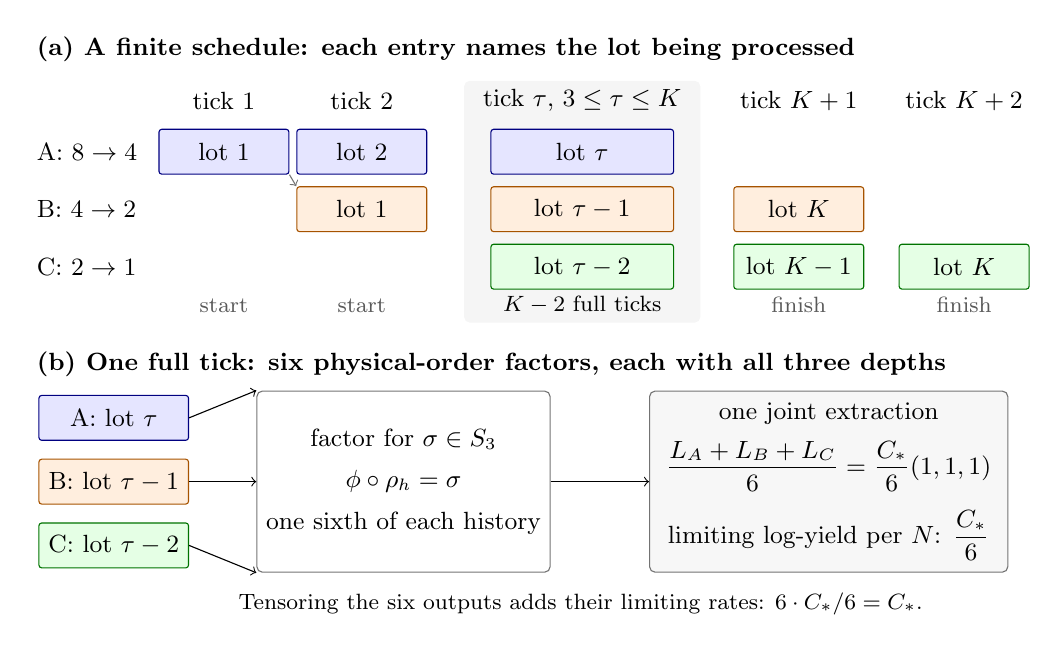
\begin{tikzpicture}[x=1cm,y=1cm,font=\small,
  stageA/.style={fill=blue!10,draw=blue!50!black},
  stageB/.style={fill=orange!13,draw=orange!65!black},
  stageC/.style={fill=green!10,draw=green!45!black},
  cell/.style={minimum height=.57cm,minimum width=1.65cm,
               rounded corners=1pt,inner sep=3pt,align=center}]
\node[anchor=west,font=\bfseries\small] at (0,0.65)
  {(a) A finite schedule: each entry names the lot being processed};
\fill[black!4,rounded corners=2pt] (5.55,-2.82) rectangle (8.55,0.25);
\node at (2.50,0) {tick $1$};
\node at (4.25,0) {tick $2$};
\node[align=center] at (7.05,0) {tick $\tau$, $3\leq\tau\leq K$};
\node at (9.80,0) {tick $K+1$};
\node at (11.90,0) {tick $K+2$};
\node[anchor=west] at (0,-.65) {A: $8\to4$};
\node[anchor=west] at (0,-1.38) {B: $4\to2$};
\node[anchor=west] at (0,-2.11) {C: $2\to1$};
\node[cell,stageA] (a1) at (2.50,-.65) {lot $1$};
\node[cell,stageA] at (4.25,-.65) {lot $2$};
\node[cell,stageA,minimum width=2.32cm] at (7.05,-.65) {lot $\tau$};
\node[cell,stageB] (b1) at (4.25,-1.38) {lot $1$};
\node[cell,stageB,minimum width=2.32cm] at (7.05,-1.38) {lot $\tau-1$};
\node[cell,stageB] at (9.80,-1.38) {lot $K$};
\node[cell,stageC,minimum width=2.32cm] (cfull) at (7.05,-2.11) {lot $\tau-2$};
\node[cell,stageC] at (9.80,-2.11) {lot $K-1$};
\node[cell,stageC] at (11.90,-2.11) {lot $K$};
\draw[->,thin,black!55] (a1.south east) -- (b1.north west);
\node[font=\footnotesize,black!65] at (2.50,-2.60) {start};
\node[font=\footnotesize,black!65] at (4.25,-2.60) {start};
\node[font=\footnotesize] at (7.05,-2.60) {$K-2$ full ticks};
\node[font=\footnotesize,black!65] at (9.80,-2.60) {finish};
\node[font=\footnotesize,black!65] at (11.90,-2.60) {finish};

\node[anchor=west,font=\bfseries\small] at (0,-3.35)
 {(b) One full tick: six physical-order factors, each with all three depths};
\node[cell,stageA,minimum width=1.90cm] (aa) at (1.10,-4.03)
 {A: lot $\tau$};
\node[cell,stageB,minimum width=1.90cm] (bb) at (1.10,-4.84)
 {B: lot $\tau-1$};
\node[cell,stageC,minimum width=1.90cm] (cc) at (1.10,-5.65)
 {C: lot $\tau-2$};
\node[draw=black!55,rounded corners=2pt,align=center,
      minimum width=3.12cm,minimum height=2.30cm] (order)
 at (4.78,-4.84)
 {factor for $\sigma\in S_3$\\[4pt]
  $\phi\circ\rho_h=\sigma$\\[4pt]
  one sixth of each history};
\draw[->] (aa.east) -- (order.north west);
\draw[->] (bb.east) -- (order.west);
\draw[->] (cc.east) -- (order.south west);
\node[draw=black!55,fill=black!3,rounded corners=2pt,align=center,
      minimum width=4.55cm,minimum height=2.30cm] (joint)
 at (10.18,-4.84)
 {one joint extraction\\[5pt]
  $\displaystyle\frac{L_A+L_B+L_C}{6}
      =\frac{C_*}{6}(1,1,1)$\\[6pt]
  limiting log-yield per $N$: $\displaystyle\frac{C_*}{6}$};
\draw[->] (order.east) -- (joint.west);
\node[align=center,font=\footnotesize] at (7.03,-6.39)
 {Tensoring the six outputs adds their limiting rates: $6\cdot C_*/6=C_*$.};
\end{tikzpicture}
\caption{Mixed-depth extraction with finite boundaries ($K\geq2$).
A lot advances one stage per tick, while a full tick combines three
different lots.  Within each physical-order factor, the common order
$\sigma$ permits one application of Theorem~\ref{thm:joint-step} to
the summed capacities.  The four boundary ticks have the positive
minima appearing in \eqref{eq:boundary-deficit}; they incur only the
fixed deficit $\beta$.  The middle column is absent when $K=2$.}
\label{fig:pipeline}
\end{figure}


Finished matrix factors are carried through subsequent operations by
tensor product.  After the last tick, every lot has terminated, and
exact coarse counts fix the number of terminal factors in every oriented
history class.  The next section computes their dimensions and then
combines that count with the yield $K(H_0+C_*)-\beta$ to obtain the rank
constraint.
